\documentclass[12pt,a4paper]{article}
\usepackage{amsmath}
\usepackage{amssymb}  % Provides \mathbb and other symbols
\usepackage{graphicx}
\usepackage{subcaption}
\usepackage{enumitem}
\usepackage{listings}
\usepackage{hyperref}
\usepackage{ulem}
\usepackage{xcolor}
\usepackage{amsthm}
\usepackage{tcolorbox}  % For colored boxes
\usepackage[table]{xcolor} % For coloring table cells
\usepackage{array}         % For better table alignment
\usepackage{mdframed}
\usepackage{cancel}
\usepackage[margin=2.5cm]{geometry}
\setlength{\parindent}{0pt}
\setlength{\parskip}{0.8em}

\begin{document}
\begin{titlepage}
\centering
\vspace*{\fill}
{\Huge Analysis III} \\[0.5cm]
{\Huge Home Work 2}\\[1.5cm]
{\Large Student: 26-712-224}\\[0.5cm]
{\Large \today}
\vspace*{\fill}
\end{titlepage}

\newpage

\noindent\textbf{Exercise 1 (Step functions, 1+2+1 P.)}\\
Let us define, for \(x\in[0;1]\),
\begin{align*}
f(x)=\sum_{k=0}^{+\infty}\chi_{[2^{-k-1},2^{-k}]}(x).
\end{align*}
(a) Is \(f\) a step function? Justify your answer briefly (you do not need to give a complete proof).

(b) Show that there exists a step function \(g:[0;1]\to\mathbb{R}\) with \(f=g\) almost everywhere and explicitly write down the set
\begin{align*}
\{x\in[0;1]:f(x)\ne g(x)\}.
\end{align*}
(c) Compute \(\int_0^1 f(x)\,dx\) by making use of (b).

\vspace{1cm}
\noindent
Answer:\\
\\
(a) $f(x)$ is NOT a valid step function.  A valid step function 
can always be represented by a finite number of bounded intervals. The sum shown is not finite and can't be repesented as as
a finite number of bounded step functions (there are infinitely many isolated points that take the value 2).\\
\\
(b) The simple step function: $g:[0, 1] \to \mathbb{R}$ given by: $g(x) = \chi_{[0,1]}(x)$ is such that $f=g$ (a.e.).\\
Now the ends of the each interval: $\chi_{[2^{-k-1},2^{-k}]}$ are "double counted" - except for\\
$k=0 \text{ when } \chi_{[2^{-k-1},2^{-k}]} = \chi_{[\frac{1}{2},1]}$.\\
Consequently, the points where $f \ne g$ is the set:
$$ D = \left\{ \frac{1}{2^k} \; \ \; k \in \mathbb{N}_{+} \right\} \cup \{0\} $$
Not that $D$ is countable and hence a set of measure zero.  I.e. $f=g$ (a.e).\\
 \\
(c) It is clear that $g$ is Lebesgue Integrable.\\
Using Theorem 11.2.15 in the notes we can conclude that, for Lebesgue Integration:\\
$$\int g = \int f$$
As $\int g = \lambda([0,1]) = 1$, we can conclude that:
$$\int f = 1$$



\newpage
\noindent\textbf{Exercise 2 (Sequences of step functions, 2+1+2+1 P.)}

\noindent Let $I$ be a compact interval in $\mathbb{R}^n$.
\begin{enumerate}
\item[(a)] Let $f:I^\circ\to\mathbb{R}$ be continuous and defined on the interior $I^\circ$ of $I$. Assuming that $f$ is unbounded from below, show that there cannot exist an increasing sequence $(f_k)_{k\in\mathbb{N}}\in T^{\mathrm{inc}}$ of step functions with $f_k\to f$ almost everywhere.
\item[(b)] Let $(f_k)_{k\in\mathbb{N}}\in T^{\mathrm{dec}}$ be a decreasing sequence of step functions for which $f_k\to\chi_I$ almost everywhere. Show that
\begin{align*}
\int_I f_k(x)\,dx\to\lambda_n(I)
\end{align*}
by reducing the problem to an application of Theorem 11.2.10(1).
\item[(c)] Consider the sequence of step functions $f_k:[0;1]\to\mathbb{R}$ given by
\begin{align*}
f_k(x)=k\chi_{[0;1/k]}(x).
\end{align*}
Prove that $f_k\to 0$ pointwise almost everywhere and compute $\int_0^1 f_k(x)\,dx$ for every $k\in\mathbb{N}$. Why is this not in contradiction with Theorem 11.2.10(1)?
\item[(d)] Let $f,g:I\to\mathbb{R}$ be two functions so that $f=g$ almost everywhere. Show that if $f\in\mathcal{L}^{\mathrm{inc}}$, then also $g\in\mathcal{L}^{\mathrm{inc}}$ and
\begin{align*}
\int_I f(x)\,dx=\int_I g(x)\,dx.
\end{align*}
\end{enumerate}

\vspace{1cm}
\noindent
Answer:\\
\\
(a) Suppose such an increasing sequence $(f_k)$ exists.
Since $f_1$ is a step function, there is $K\in\mathbb{R}$
such that $f_1(x)\geq K$ everywhere. Thus
\begin{align*}
f_k(x)\geq f_1(x)\geq K.
\end{align*}
Taking limits gives $f(x)\geq K$ almost everywhere.

Since $f$ is unbounded below, choose $x_0\in I^\circ$
with $f(x_0)<K$. By continuity, there exists $r>0$
such that $B(x_0,r)\subset I^\circ$ and
\begin{align*}
f(x)<K\qquad\text{for every }x\in B(x_0,r).
\end{align*}
This ball has positive measure, contradicting
$f\geq K$ almost everywhere. Therefore no such
sequence exists.\\
\\
(b) Define the step functions
\begin{align*}
h_k=(f_k-\chi_I)\chi_I.
\end{align*}
Then $(h_k)$ is decreasing and $h_k\to0$
almost everywhere. By Theorem 11.2.10(1),
\begin{align*}
\int h_k(x)\,dx\longrightarrow0.
\end{align*}
Therefore
\begin{align*}
\int_I f_k(x)\,dx
&=\int h_k(x)\,dx+\int_I 1\,dx\\
&=\int h_k(x)\,dx+\lambda_n(I)
\longrightarrow\lambda_n(I).
\end{align*}
\\
(c)
Fix $x\in(0,1]$. Choose $K>1/x$.
For every $k\geq K$, $1/k<x$, so $f_k(x)=0$.
Thus $f_k(x)\to0$ for every $x>0$.
At $x=0$, $f_k(0)=k\to+\infty$.
Since $\{0\}$ is null, convergence holds almost everywhere.

For every $k\geq1$,
\begin{align*}
\int_0^1 f_k(x)\,dx
=k\,\lambda([0,1/k])=k\frac1k=1.
\end{align*}
There is no contradiction with Theorem 11.2.10(1):
the sequence is not decreasing. Indeed,
\begin{align*}
f_{k+1}(x)=k+1>k=f_k(x)
\qquad\text{for }0<x<\frac1{k+1}.
\end{align*}

\newpage
\noindent
\textbf{Exercise 3 - Non-integrable function}

Consider
\begin{align*}
f(x)=\frac{1}{x}
\end{align*}
for $x\in(0;1]$.

\begin{enumerate}
\item[(a)] Construct an increasing sequence
$(f_k)_{k\in\mathbb{N}}\in T^{\mathrm{inc}}$
of step functions on $(0;1]$ so that $f_k\to f$
almost everywhere.

\item[(b)] Let $(g_k)_{k\in\mathbb{N}}\in T^{\mathrm{inc}}$
be any increasing sequence of step functions with
$g_k\to f$ almost everywhere. Show that the sequence
\begin{align*}
\left(\int_0^1 g_k(x)\,dx\right)_{k\in\mathbb{N}} \tag{3.1}
\end{align*}
is unbounded. Is $f\in\mathcal{L}^{\mathrm{inc}}$?
\end{enumerate}

\vspace{1cm}
\noindent
Answer:\\
\\
(3)(a) This idea is copied from our lecture.\\
\\
I have show a graph of the region (approx) we are interested in (with $x \in (0,1]$).
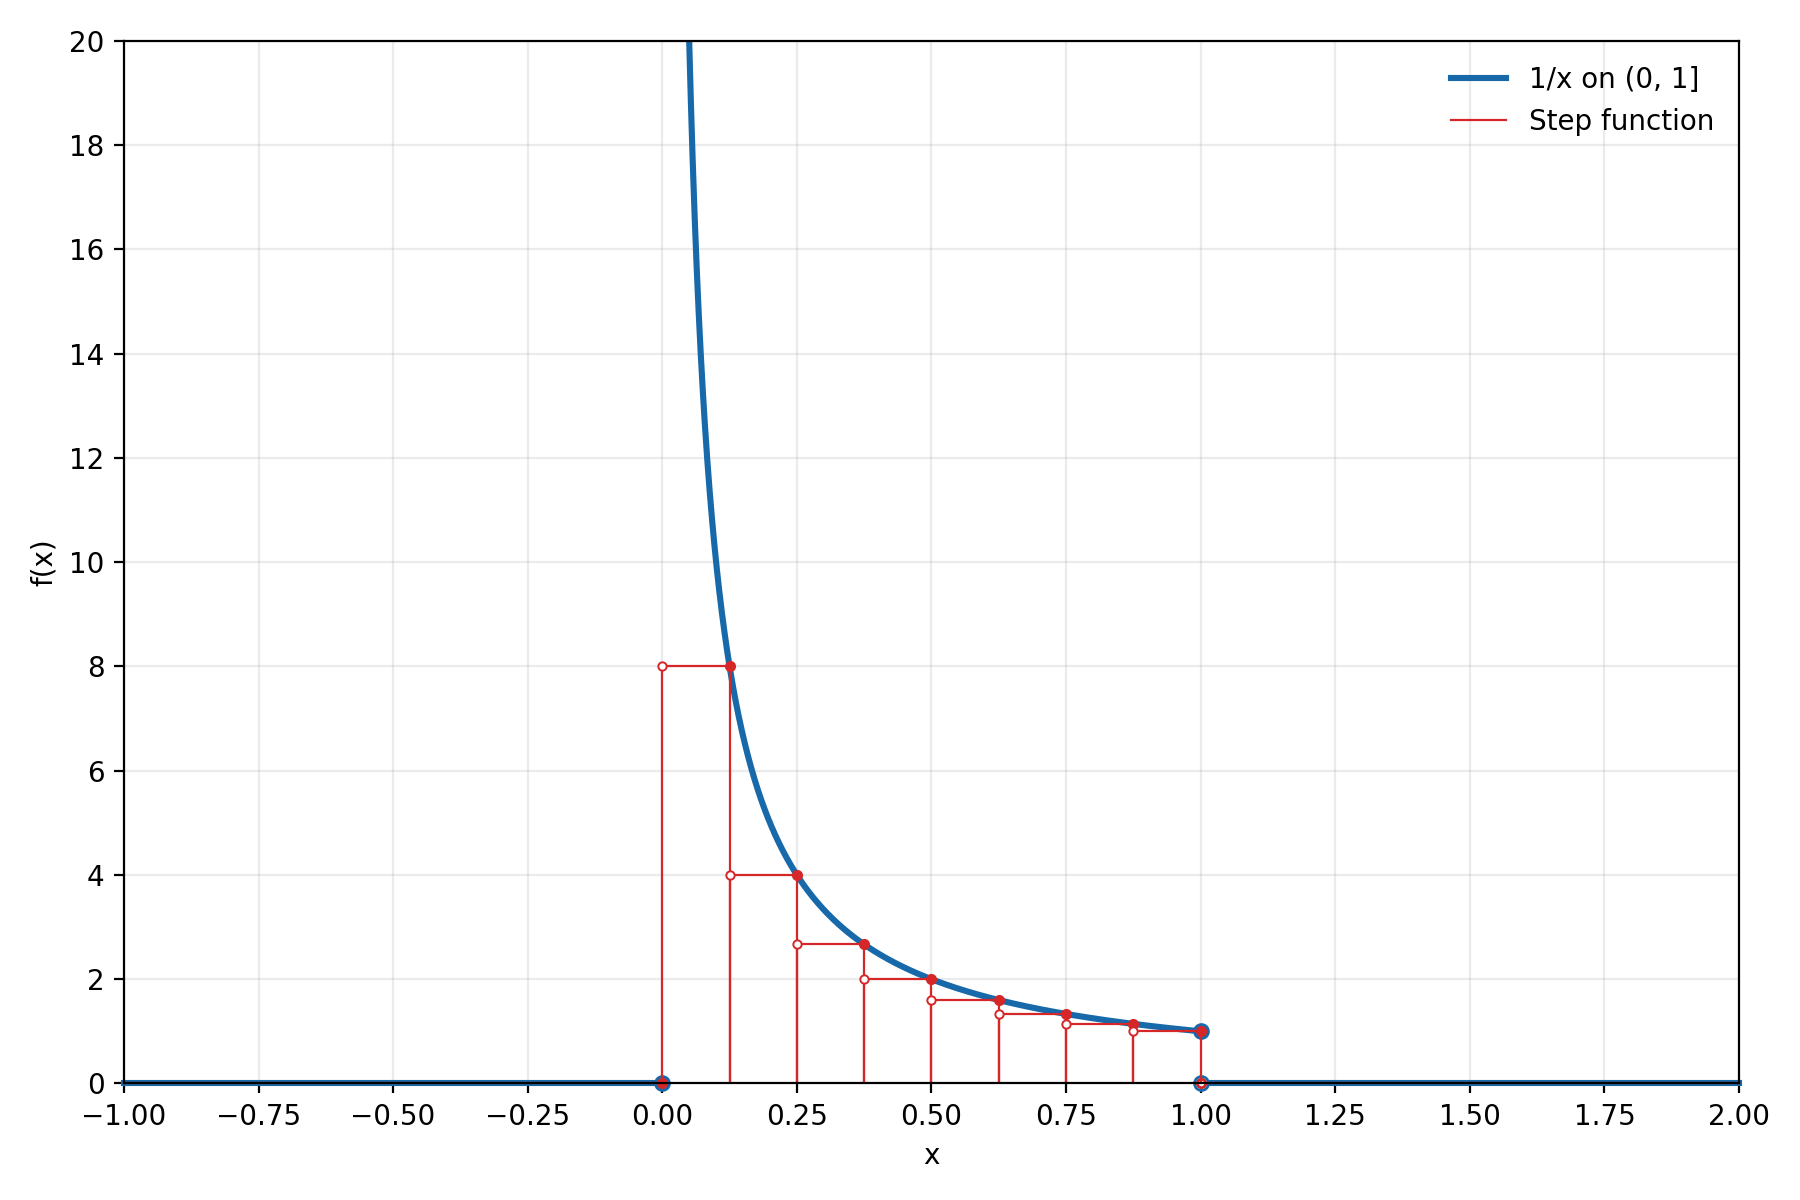
\includegraphics[width=\textwidth]{Diagrams/ANAL_III_WK_2_Q3.png}
The red rectangles are the step function:
\begin{align*}
f_k(x)=
\begin{cases}
0, & x\leq 0,\\
\dfrac{N_k}{j}, &
x\in\left(\dfrac{j-1}{N_k},\dfrac{j}{N_k}\right],
\quad j=1,\ldots,N_k,\\
0, & x>1,
\end{cases}
\end{align*}
where $N_k=2^k$. \\
\\
In the graph I have plotted $f_3(x)$.  Monotonicity is obvious and $(f_k)_{k \in \mathbb{N}} \in T^{inc}((0,1],\mathbb{R}_{>0})$.\\
Let's prove pointwise convergence:\\
Fix $x\in(0,1]$. Let $b_k$ be the right endpoint
of the interval containing $x$. Then
\begin{align*}
0 &\leq b_k-x<2^{-k}, &
f_k(x)&=\frac{1}{b_k}.
\end{align*}
Therefore
\begin{align*}
0\leq \frac{1}{x}-f_k(x)
&=\frac{b_k-x}{xb_k}
\leq \frac{2^{-k}}{x^2}
\longrightarrow 0.
\end{align*}
Hence $f_k(x)\to 1/x$.\\
\\
(b) We have proved (in lectures) the following theorem:

\textbf{Theorem 11.2.10 (1)}
Let $(f_k)_{k\in\mathbb{N}}\subset T$ be a
monotonically decreasing sequence of step functions
with $f_k\xrightarrow{k\to\infty}0$ a.e. in
$\mathbb{R}$. Then:
\begin{align*}
\lim_{k\to\infty}\int f_k=0.
\end{align*}
We shall show that the limit of this Lebesgue integral does NOT exist for our $(f_k)_k$ from part (a).\\
\\
For each of the $N_k=2^k$ rectangles, the area is:
\begin{align*}
\frac{1}{2^k}\frac{2^k}{j}=\frac{1}{j}.
\end{align*}
Hence the total area is:
\begin{align*}
A_k=\sum_{j=1}^{2^k}\frac{1}{j}.
\end{align*}
This is a well known series and diverges as
$k\to+\infty$.

Now let $(g_k)_{k\in\mathbb{N}}\in T^{\mathrm{inc}}$
be any increasing sequence of step functions with
$g_k\to f$ almost everywhere.

Fix $A>0$. Since $A_m\to+\infty$, choose $m$ such that
\begin{align*}
\int_0^1 f_m(x)\,dx=A_m>A+1.
\end{align*}
Keep $m$ fixed and define
\begin{align*}
h_k=\max(f_m-g_k,0).
\end{align*}
Each $h_k$ is a step function. Since $g_k$ increases
to $f$ almost everywhere and $f_m\leq f$,
$h_k$ decreases to $0$ almost everywhere.
By Theorem 11.2.10(1),
\begin{align*}
\int_0^1 h_k(x)\,dx\longrightarrow 0.
\end{align*}
Thus there exists $K$ such that, for every $k\geq K$,
\begin{align*}
\int_0^1 h_k(x)\,dx<1.
\end{align*}
Since $f_m\leq g_k+h_k$, for every $k\geq K$,
\begin{align*}
\int_0^1 g_k(x)\,dx
&\geq \int_0^1 f_m(x)\,dx-\int_0^1 h_k(x)\,dx\\
&>A.
\end{align*}
Since $A>0$ was arbitrary,
\begin{align*}
\int_0^1 g_k(x)\,dx\longrightarrow+\infty.
\end{align*}
Therefore the sequence is unbounded, and
$f\notin\mathcal{L}^{\mathrm{inc}}$.

\end{document}